\section{Ricostruzione delle fessure}
\label{sec:gap_reconstruction}

\subsection{Ricostruzione porte}

Consideriamo il caso più semplice, ovvero le porte. L'obiettivo è prendere i soli segmenti relativi alle porte e ricostruire, per ciascuno di essi, la faccia chiusa corrispondente, sfruttando la struttura spaziale e la lista degli archi (\texttt{edge}) costruite nella fase precedente.

Ricordiamo che la procedura di snapping è stata eseguita esclusivamente sui segmenti dei muri: al suo termine abbiamo quindi a disposizione l'hash spaziale e una lista di archi, dove ogni arco è rappresentato da due indici di vertice e da un tag che ne descrive il tipo (\texttt{WALL}/\texttt{DOOR}/\texttt{WINDOW}). A questo punto, sia i vertici presenti nell'hash sia gli archi della lista appartengono esclusivamente ai muri:
\begin{minted}[frame=single]{cpp}
struct Edge
{
  VertexId v1, v2;
  SegmentLayer layer;
};

struct SnappingResult
{
  SpatialHash hash;
  std::vector<Edge> edges;
};
\end{minted}

L'idea è di iterare su ogni segmento delle porte e, per ciascuno, considerarne i due vertici estremi. Invece di creare due nuovi vertici, sfruttiamo il fatto che una porta collega sempre gli spigoli di due muri: tramite il metodo

\begin{minted}{cpp}
	VertexId find_nearest(glm::dvec2 p)
\end{minted}

recuperiamo i due vertici dei muri corrispondenti a quella specifica porta, senza duplicarli, e aggiungiamo un nuovo arco tra di essi con tag \texttt{DOOR}.

Una porta, tuttavia, non è rappresentabile con un singolo segmento: è una faccia rettangolare chiusa, delimitata da due segmenti paralleli. Questo concetto risulterà più chiaro nella sezione dedicata all'estrazione e alla classificazione delle facce. Ci servono quindi altri due vertici per individuare il secondo segmento, parallelo al primo. Consideriamo lo scenario di Figura~\ref{fig:wall_graph}.

\begin{figure}[htbp]
	\centering
	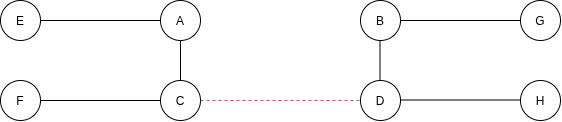
\includegraphics[width=0.5\textwidth]{images/02_geometry_processing/wall_graph.png}
	\caption{Singolo segmento}
	\label{fig:wall_graph}
\end{figure}

Sia $\vec{CD}$ il segmento noto, dove $C$ e $D$ sono le due giunzioni con i muri. Il nodo $C$ è collegato, tramite archi \texttt{WALL} già esistenti, ai soli vicini $A$ e $F$; analogamente, il nodo $D$ è collegato a $B$ e $H$. Per individuare quale dei due vicini di $C$ appartenga al segmento parallelo cercato, si calcola il prodotto scalare tra i versori (vettori normalizzati) di $\vec{CD}$ e di ciascun vicino: un valore prossimo a $0$ indica perpendicolarità tra i due segmenti. Applicando questo criterio ai vicini di $C$: il vettore $\vec{CF}$ risulta pressoché opposto a $\vec{CD}$ (prodotto scalare $\approx -1$) e viene scartato; il vettore $\vec{CA}$ risulta invece perpendicolare a $\vec{CD}$ (prodotto scalare $\approx 0$), individuando così il primo vertice candidato, $A$.
Ripetendo lo stesso criterio sui vicini di $D$ ($B$ e $H$), si individua analogamente il secondo vertice candidato, $B$. Il secondo segmento cercato, parallelo a $\vec{CD}$, è quindi $\vec{AB}$ (Figura~\ref{fig:wall_graph_2}).
\begin{figure}[htbp]
	\centering
	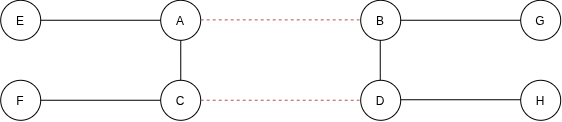
\includegraphics[width=0.5\textwidth]{images/02_geometry_processing/wall_graph_2.png}
	\caption{Doppio segmento}
	\label{fig:wall_graph_2}
\end{figure}

Per chiudere la faccia rettangolare della porta è quindi sufficiente aggiungere i due nuovi archi $\vec{CD}$ e $\vec{AB}$, entrambi con tag \texttt{DOOR}, senza dover introdurre alcun nuovo vertice.

Alla fine, ignorando per il momento le finestre, il procedimento di ricostruzione delle porte produce la rappresentazione mostrata in Figura~\ref{fig:doors}: dopo la fase di snapping disponevamo di 88 vertici e 88 archi; dopo la ricostruzione delle porte otteniamo 10 nuovi archi (98 archi totali). Il dato è coerente, poiché sono presenti 5 porte, ciascuna delle quali richiede l'aggiunta di 2 nuovi archi.
\begin{figure}[htbp]
	\centering
	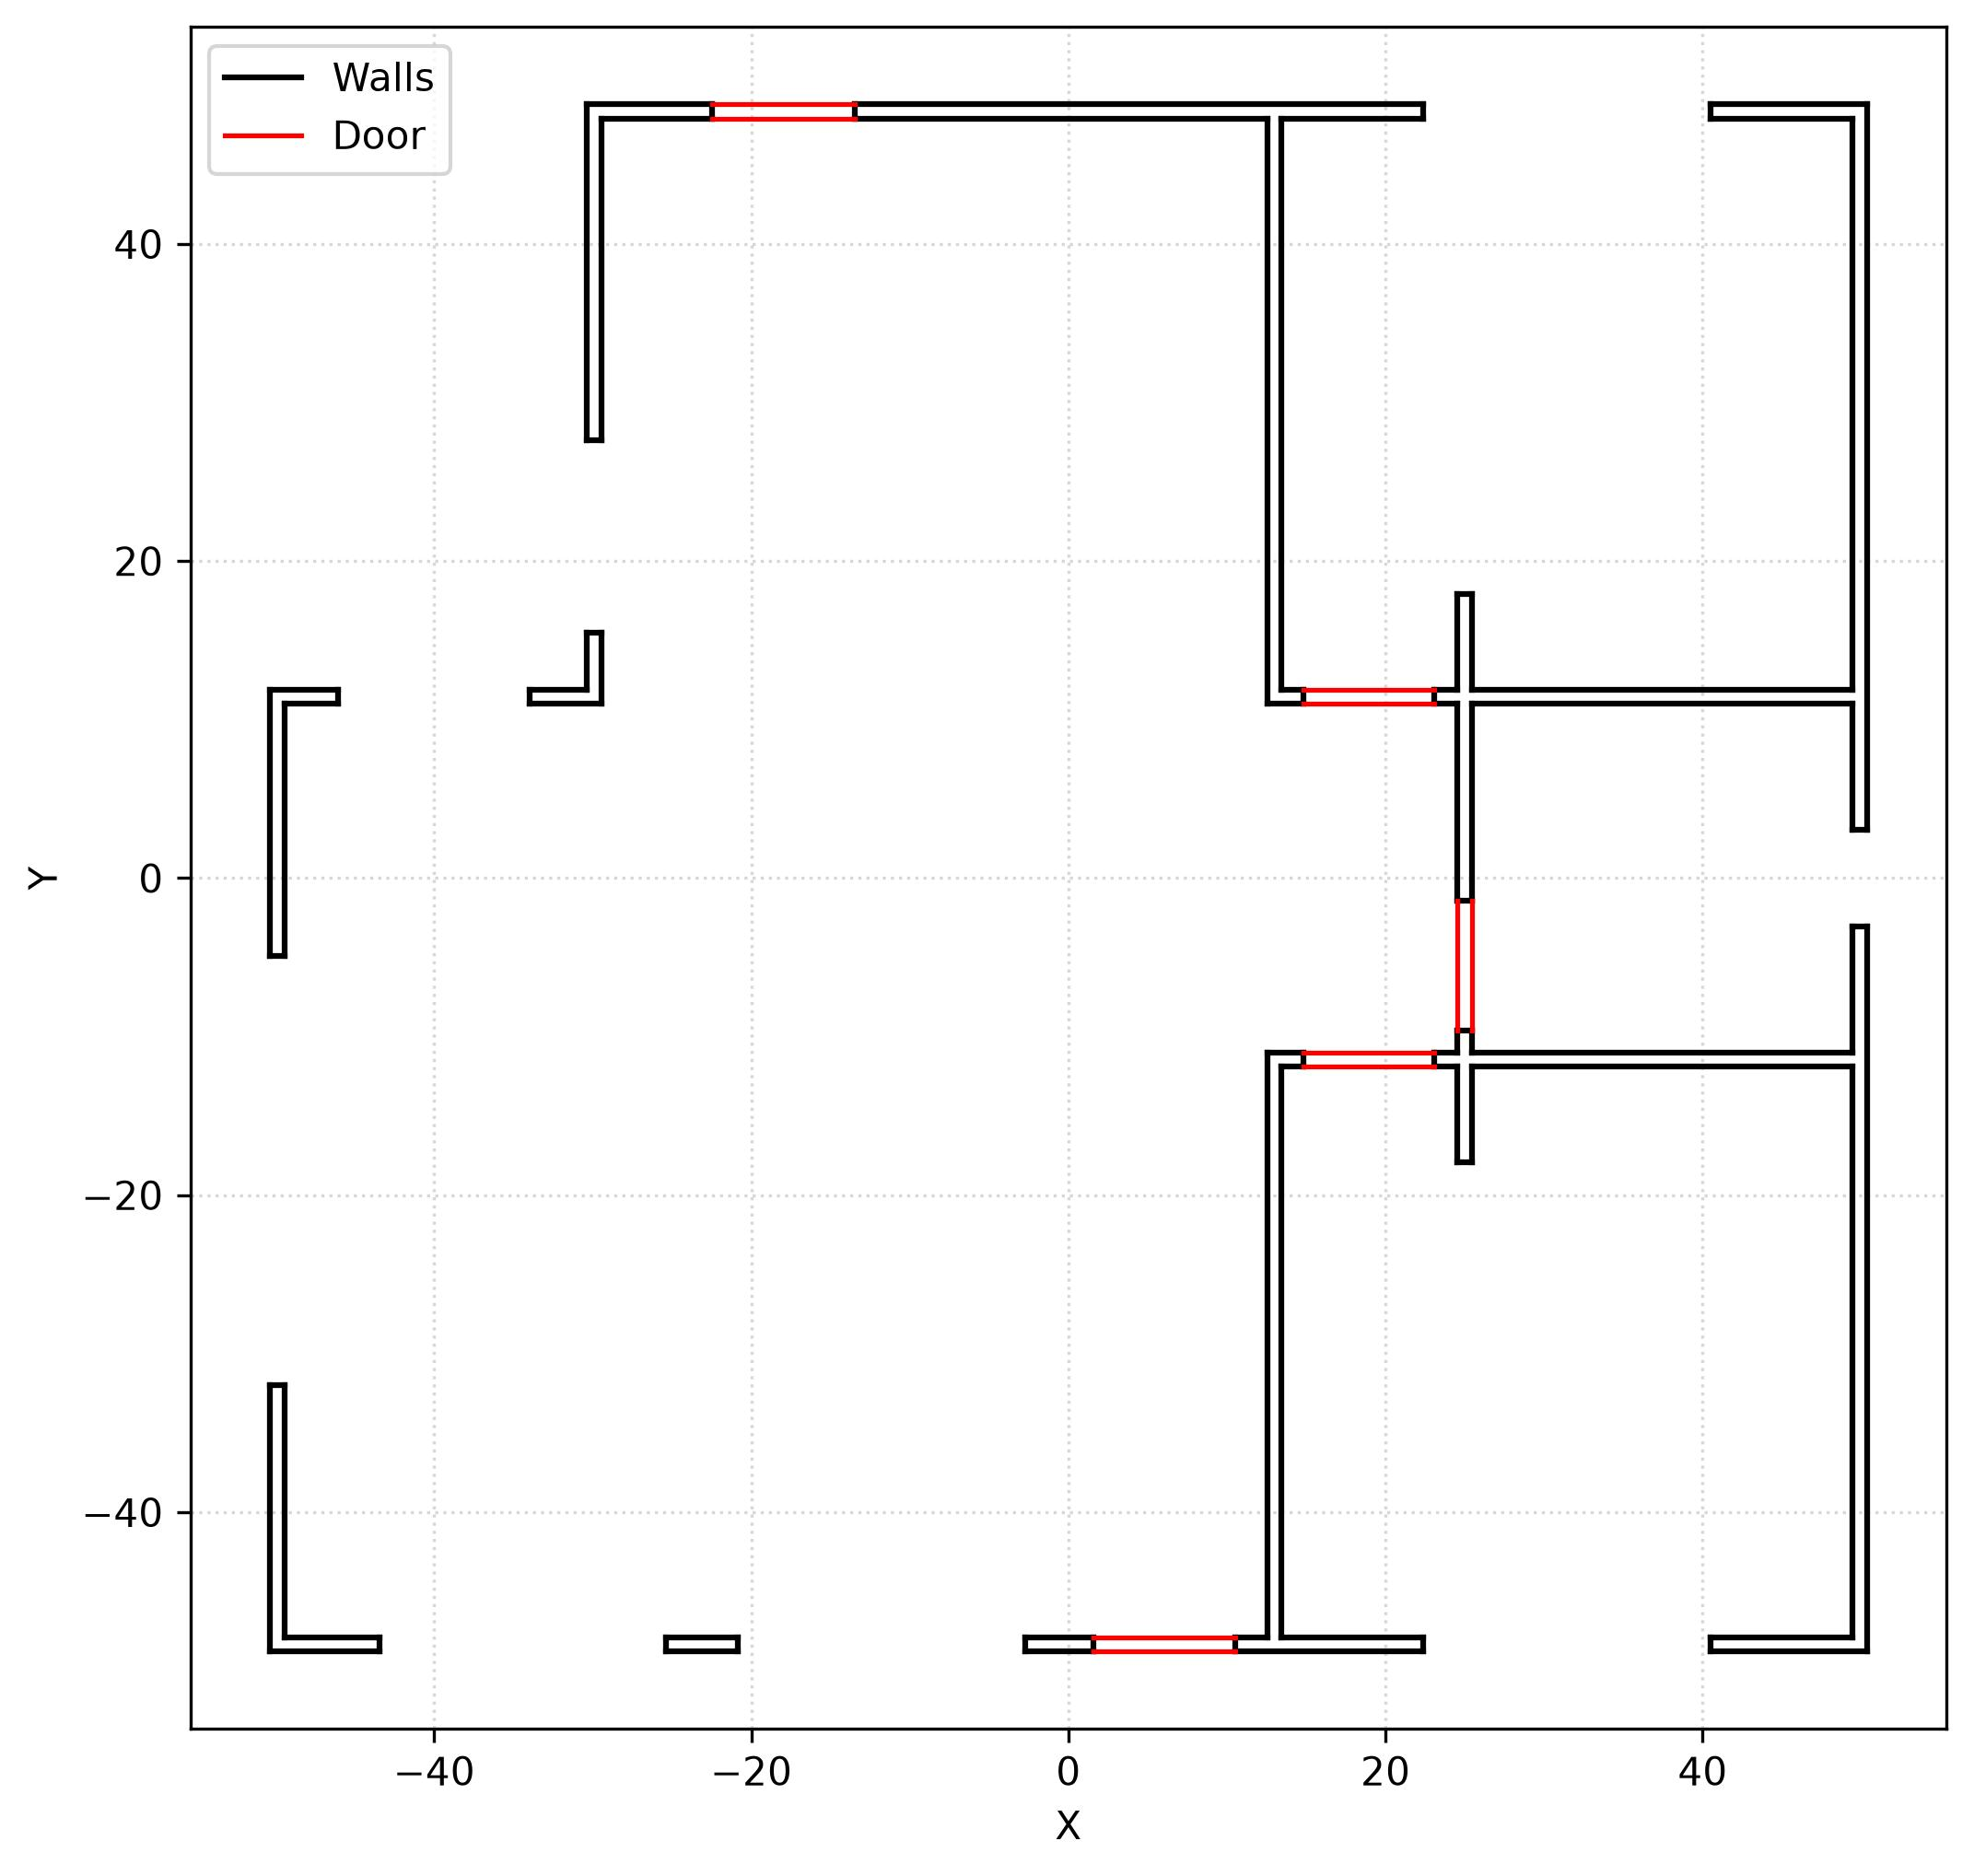
\includegraphics[width=1\textwidth]{images/02_geometry_processing/doors_connected.jpg}
	\caption{Le porte adesso sono rappresentate da due segmenti paralleli}
	\label{fig:doors}
\end{figure}


\subsection{Ricostruzione finestre}
\label{subsec:windows}

Resta da affrontare la ricostruzione delle finestre. Nel modello di caso di studio una finestra è rappresentata da decine di segmenti e punti; in altri modelli, tuttavia, le finestre possono presentarsi in forme completamente diverse. Non è possibile trattare esplicitamente ogni possibile scenario di rappresentazione, per cui è necessario un approccio più generale rispetto a quello utilizzato per le porte.

L'approccio adottato si basa sul clustering spaziale e sull'estrazione del bounding box. I punti campionati lungo i segmenti di ciascuna finestra vengono raggruppati in cluster: ogni cluster conterrà un numero variabile di punti, che non è rilevante ai fini dell'algoritmo, e rappresenterà una finestra distinta. Poiché interessa conoscere unicamente il punto di inizio e di fine di ciascuna finestra, per ogni cluster viene calcolato il bounding box, da cui si estrae uno dei due lati lunghi. Il segmento così ottenuto, che congiunge le due giunzioni con i muri, viene trattato esattamente come il segmento di partenza usato per le porte: si applica quindi lo stesso identico procedimento descritto in precedenza per ricostruire il secondo segmento parallelo e chiudere la faccia. Al termine, anche ogni finestra risulta rappresentata da una faccia chiusa.

L'algoritmo utilizzato per il clustering è DBSCAN (Density-Based Spatial Clustering of Applications with Noise) \cite{ester1996dbscan}, implementato tramite la libreria \texttt{SimpleDBSCAN}. Sarà cruciale impostare correttamente due parametri: il numero di sample generati lungo ciascun segmento di finestra (campionati in modo lineare lungo il segmento), e la distanza massima $\varepsilon$ entro cui due sample sono considerati appartenenti allo stesso cluster. È necessario valutare un compromesso tra questi due parametri: con un numero elevato di sample il costo computazionale cresce, mentre con un numero troppo basso aumenta il rumore nei cluster risultanti. Analogamente, se la tolleranza $\varepsilon$ è troppo alta si rischia che due cluster distinti finiscano per sovrapporsi; se è troppo bassa, si rischia di ottenere un cluster per ciascun punto.

\begin{figure}[htbp]
	\centering
	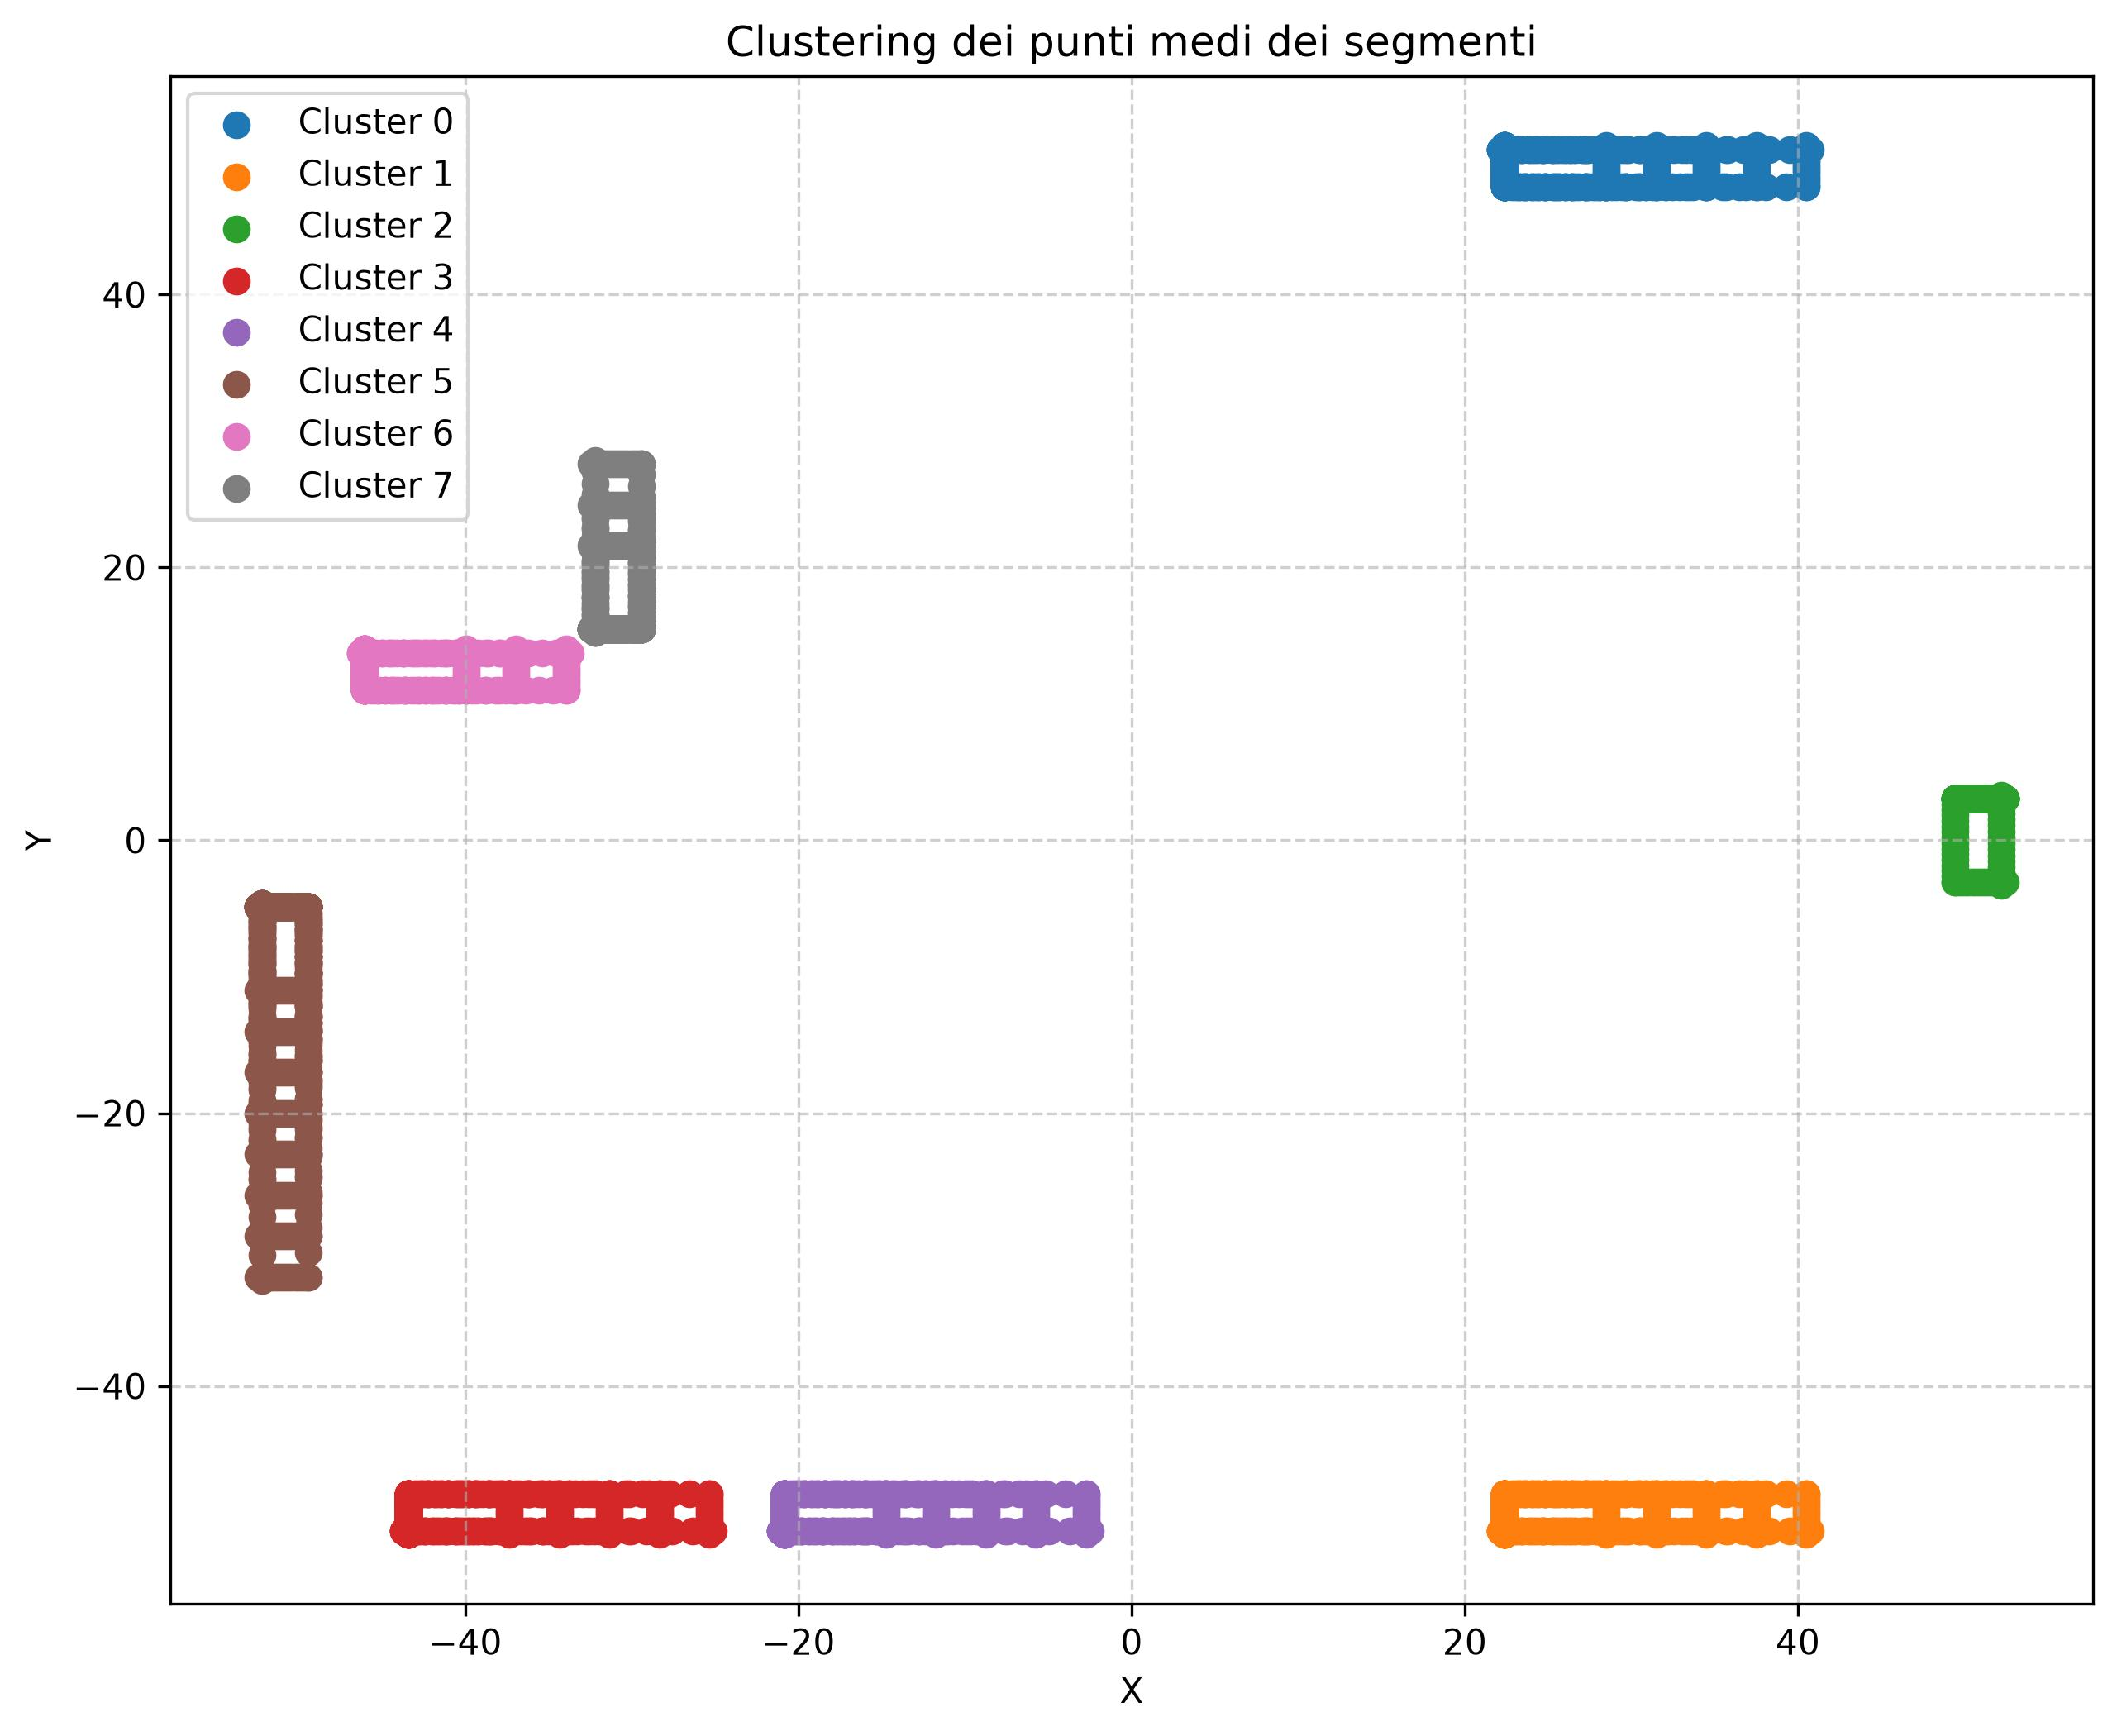
\includegraphics[width=1\textwidth]{images/02_geometry_processing/clusters.jpg}
	\caption{Nel nostro caso, con 15 sample per segmento e tolleranza $\varepsilon = 2$ otteniamo 8 cluster distinti corrispondenti alle 8 finestre presenti nel modello.}
	\label{fig:clusters}
\end{figure}

Dopo aver calcolato i bounding box e ricavato i relativi segmenti, è possibile ricostruire tutte le finestre. La rappresentazione completa di muri, porte e finestre risultante è mostrata in Figura~\ref{fig:windows_connected}.

\begin{figure}[htbp]
	\centering
	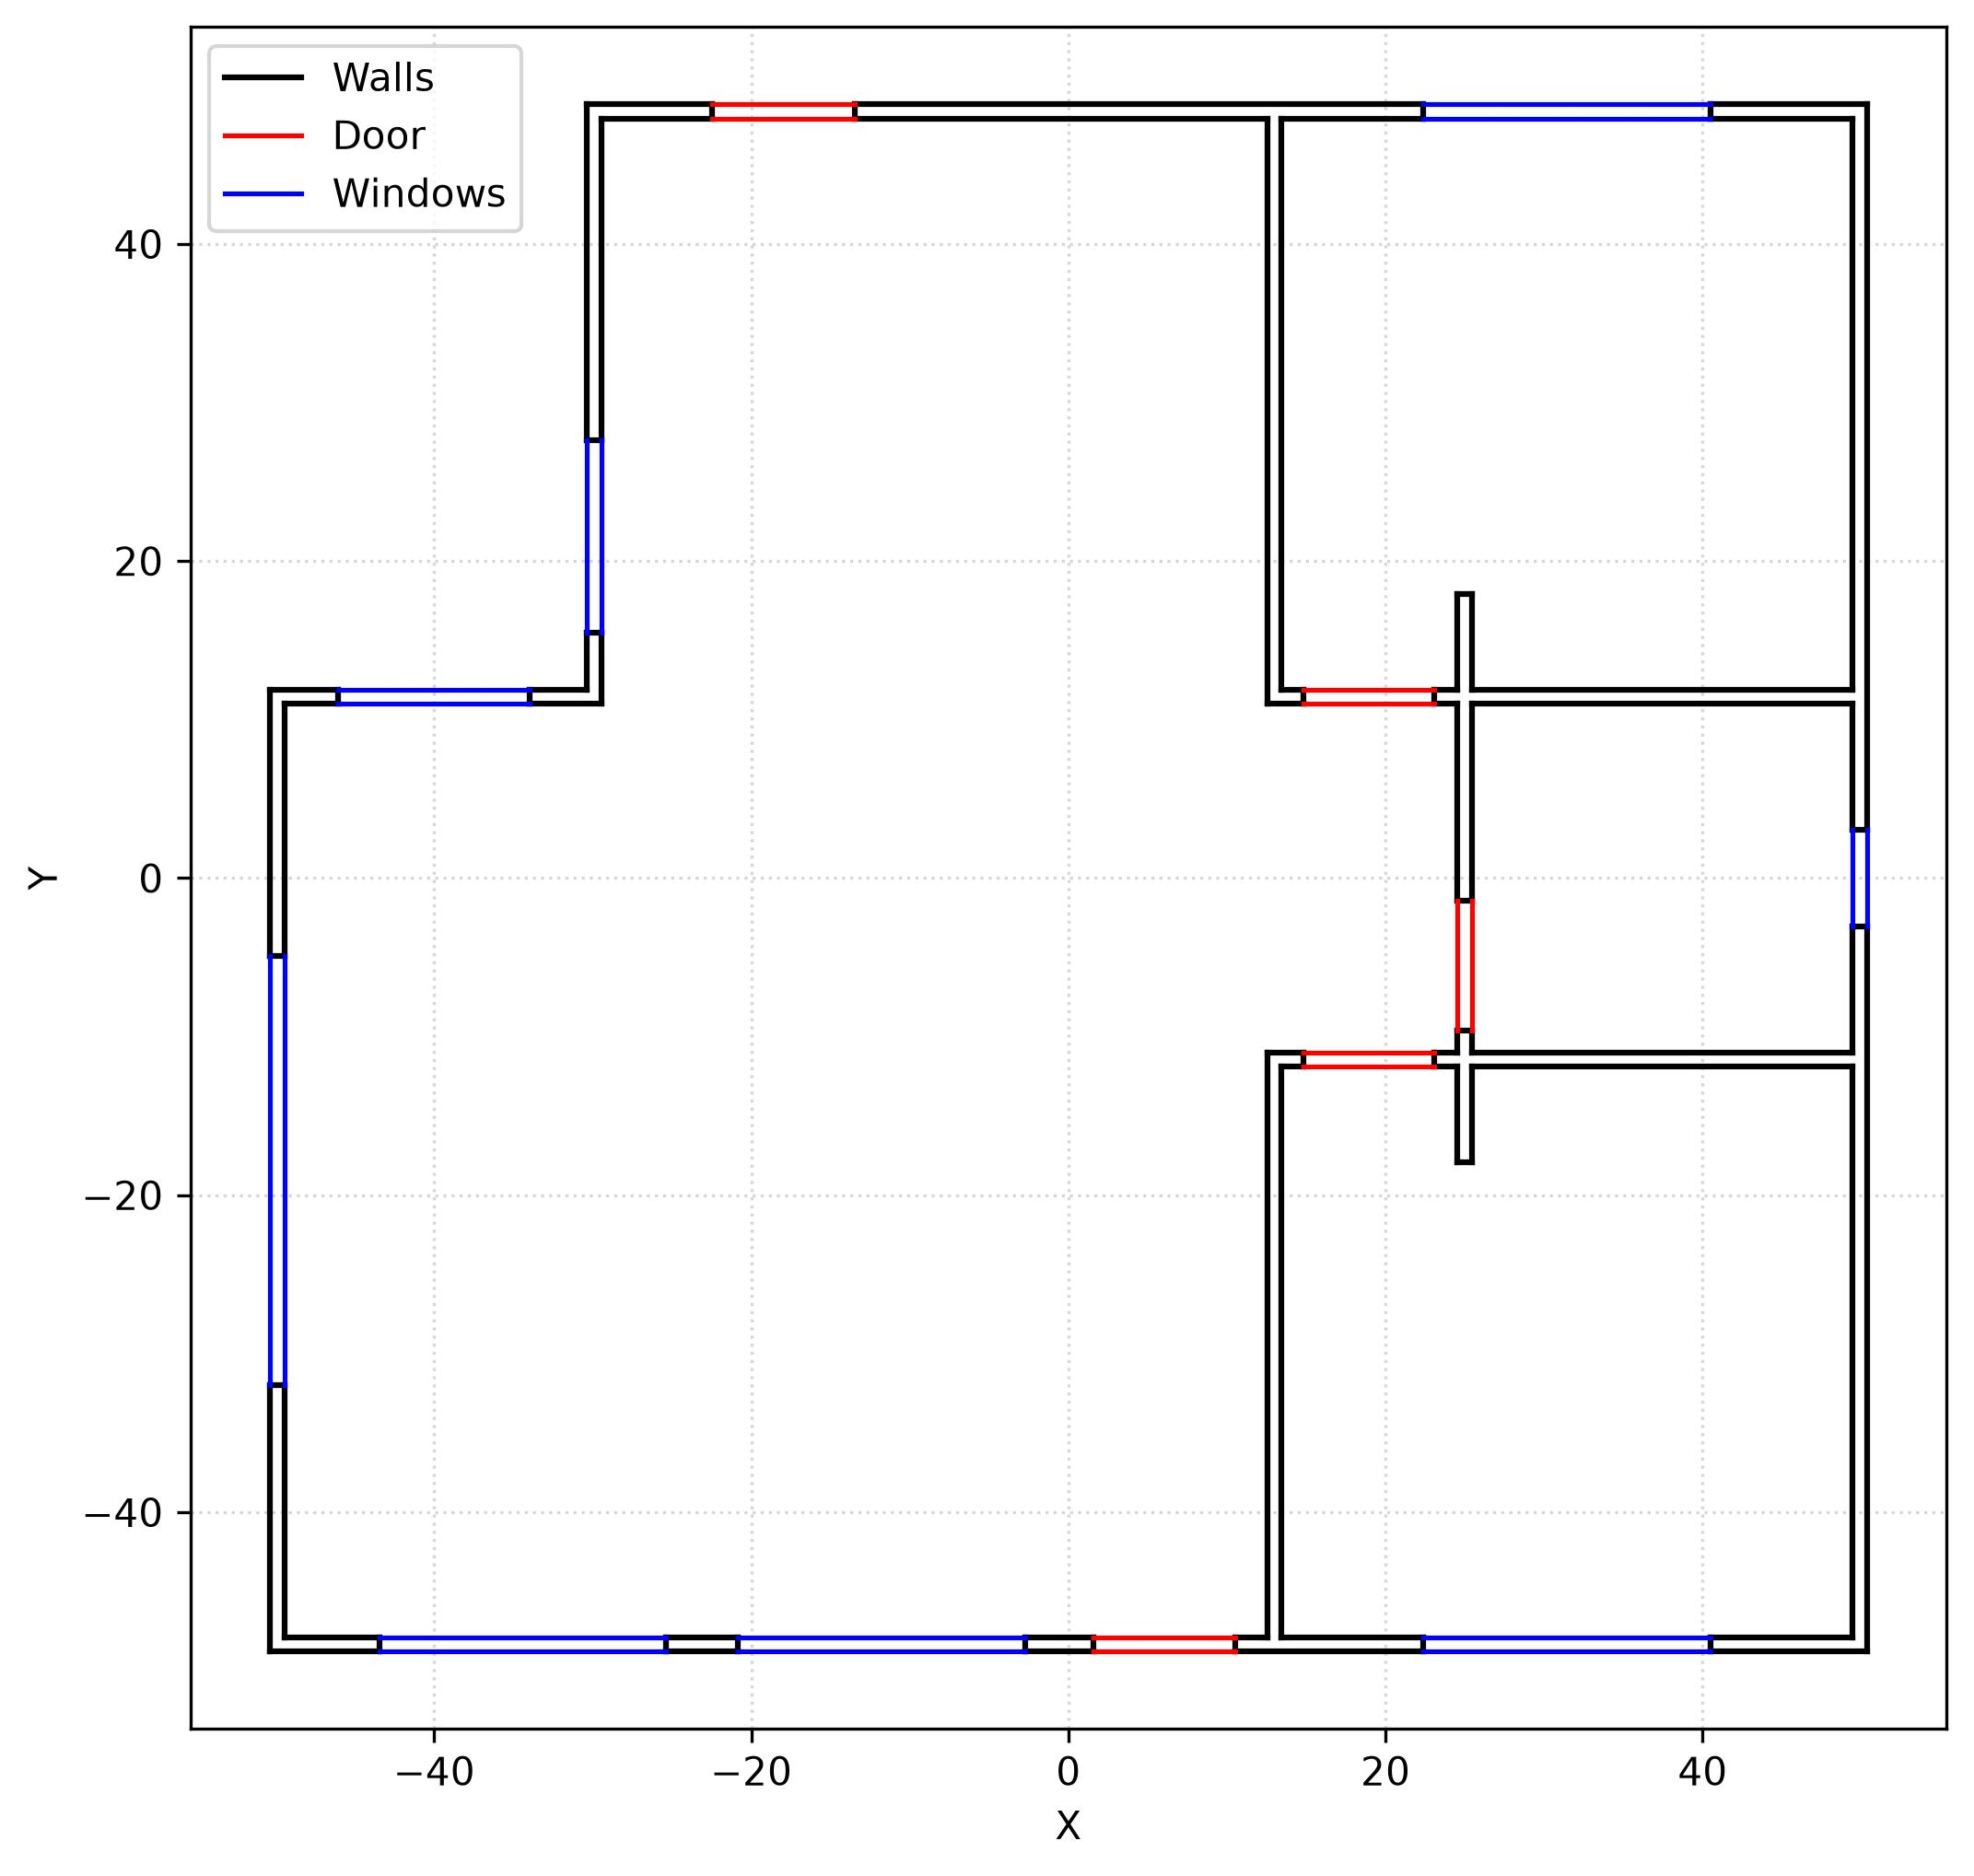
\includegraphics[width=1\textwidth]{images/02_geometry_processing/windows_connected.jpg}
	\caption{Ricostruzione completa dei varchi: muri, porte e finestre.}
	\label{fig:windows_connected}
\end{figure}

Il risultato di questa fase è un grafo completo di muri, porte e finestre, pronto per essere utilizzato nella costruzione del \emph{Planar Straight-Line Graph} e nell'estrazione delle facce.
